%!TEX root = ../ENTRUST_TR.tex

We will demonstrate the application of \approach using a self-adaptive UUV embedded system, adapted from~\cite{Gerasimou2014:SEAMS} . UUVs are increasingly used in a wide range of oceanographic and military tasks, including oceanic surveillance (e.g., to monitor pollution levels and ecosystems), undersea mapping, and mine detection. Limitations intrinsic to the environment in which these vehicles operate (e.g., impossibility  to maintain UUV-operator communication during missions and high frequency of unexpected changes) require that UUV systems are self-adaptive. These systems are also safety critical (e.g., when used for mine detection and surveillance of ecosystems that should not be impacted) and/or business critical, since UUVs are often expensive equipment that should not be lost during missions.

The self-adaptive system in our study consists of a UUV used to carry out a surveillance and data gathering mission. The UUV is equipped with $n \geq 1$ on-board sensors that can measure the same attribute of the ocean environment (e.g., water current, salinity or thermocline). When used, the sensors take measurements with different, variable rates $r_1$, $r_2$, \ldots, $r_n$. The probability that each sensor produces measurements that are sufficiently accurate for the purpose of the mission depends on the UUV speed $sp$, given by  $p_1$, $p_2$, \ldots, $p_n$\footnote{This information can be extracted from the technical specification of sensors; for example, see \url{http://www.ashtead-technology.com/rental-equipment/teledyne-rdi-600khz-navigator/}}. For each measurement taken, different amount of energy is consumed, given by $e_1$, $e_2$, \ldots, $e_n$ . % These measurements have an accuracy that depends on the UUV speed $sp$, and the (speed-dependent) probabilities $p_1$, $p_2$, \ldots, $p_n$ that the sensors produce measurements that are sufficiently accurate for the purpose of mission can be calculated from the technical specifications of the sensors. 
Finally, the $n$ sensors can be switched on and off individually (e.g., to save battery power when not required), but these operations consume an amount of energy given by $e^\mathrm{on}_1$, $e^\mathrm{on}_2$, \ldots, $e^\mathrm{on}_n$ and $e^\mathrm{off}_1$, $e^\mathrm{off}_2$, \ldots, $e^\mathrm{off}_n$, respectively.

The UUV is required to self-adapt to changes in the observed sensor measurement rates $r_i$, $1\leq i\leq n$, and to sensor failures by dynamically adjusting:
\squishlist
\item[(a)] the UUV speed $sp$
\item[(b)] the sensor configuration $x_1$, $x_2$, \ldots, $x_n$ (where $x_i=1$ if the $i$-th sensor is on and $x_i=0$ otherwise)
\squishend
so that the UUV complies with the following requirements at all times:
\squishlist
	\item[\textbf{R1}:] The UUV should take at least 20 measurements of sufficient accuracy for every 10~metres of mission distance.
	\item[\textbf{R2}:] The energy consumption of the sensors should not exceed 120 Joules per 10 surveyed metres.
	\item[\textbf{R3}:] If requirements R1 and R2 are satisfied by multiple configurations, the UUV should use one of these configurations that minimises the cost function
\begin{equation}
\label{eq:cost}
cost = w_1 E + w_2 s^{-1},
\end{equation}
where $E$ represents the energy consumed by the sensors to survey a 10m mission distance, and $w_1, w_2 >0$ represent weights that reflect the relative importance of carrying out the mission with reduced battery usage and completing the mission faster.
\squishend

\begin{example}
Figure~1 depicts the CTMC model $M_i$ of the $i$-th sensor of the UUV from our running example. The CTMC starts in state 0 and transitions in state 1 if the sensor is switched on ($x_i=1$) or in state 6 otherwise ($x_i=0$). With rate $r_i$,  a measurement is performed, as indicated by the transition between states 1 and 2. The measurement is ``sufficiently accurate" with probability $p_i$ and the transition between states 2 and 3 is taken, whereas the transition between states 2 and 4 is enabled in case of an inaccurate measurement. An active sensor continues taking measurements while it is active,  as modelled by the transition between states 5 and 1. The CTMC model is augmented with two cost/reward structures, whose non-zero elements are shown in Fig.~1 in rectangular boxes, and dashed rectangular boxes, respectively. The former, ``\textit{energy}'' structure associates the energy used to switch the sensor on (i.e., $e_i^\mathrm{on}$) and off (i.e., $e_i^\mathrm{off}$) and to perform a measurement (i.e., $e_i$) with the CTMC transitions that model these events. Note that the ternary expression ``$\mathit{condition}?a\!:\!b$'' was used to indicate that the energy $e_i^\mathrm{on}$ is consumed only if the previous state of the sensor was ``off'', i.e., if $x_i^\mathrm{old}=0$, whereas the energy $e_i^\mathrm{off}$ is used  only if the opposite is true ($x_i^\mathrm{old}=1$). As concerns the latter, ``\textit{measurement}'' cost/reward structure, it associates a reward of $1$ with the transition that corresponds to an accurate measurement. 

\begin{figure}[t]
\centering
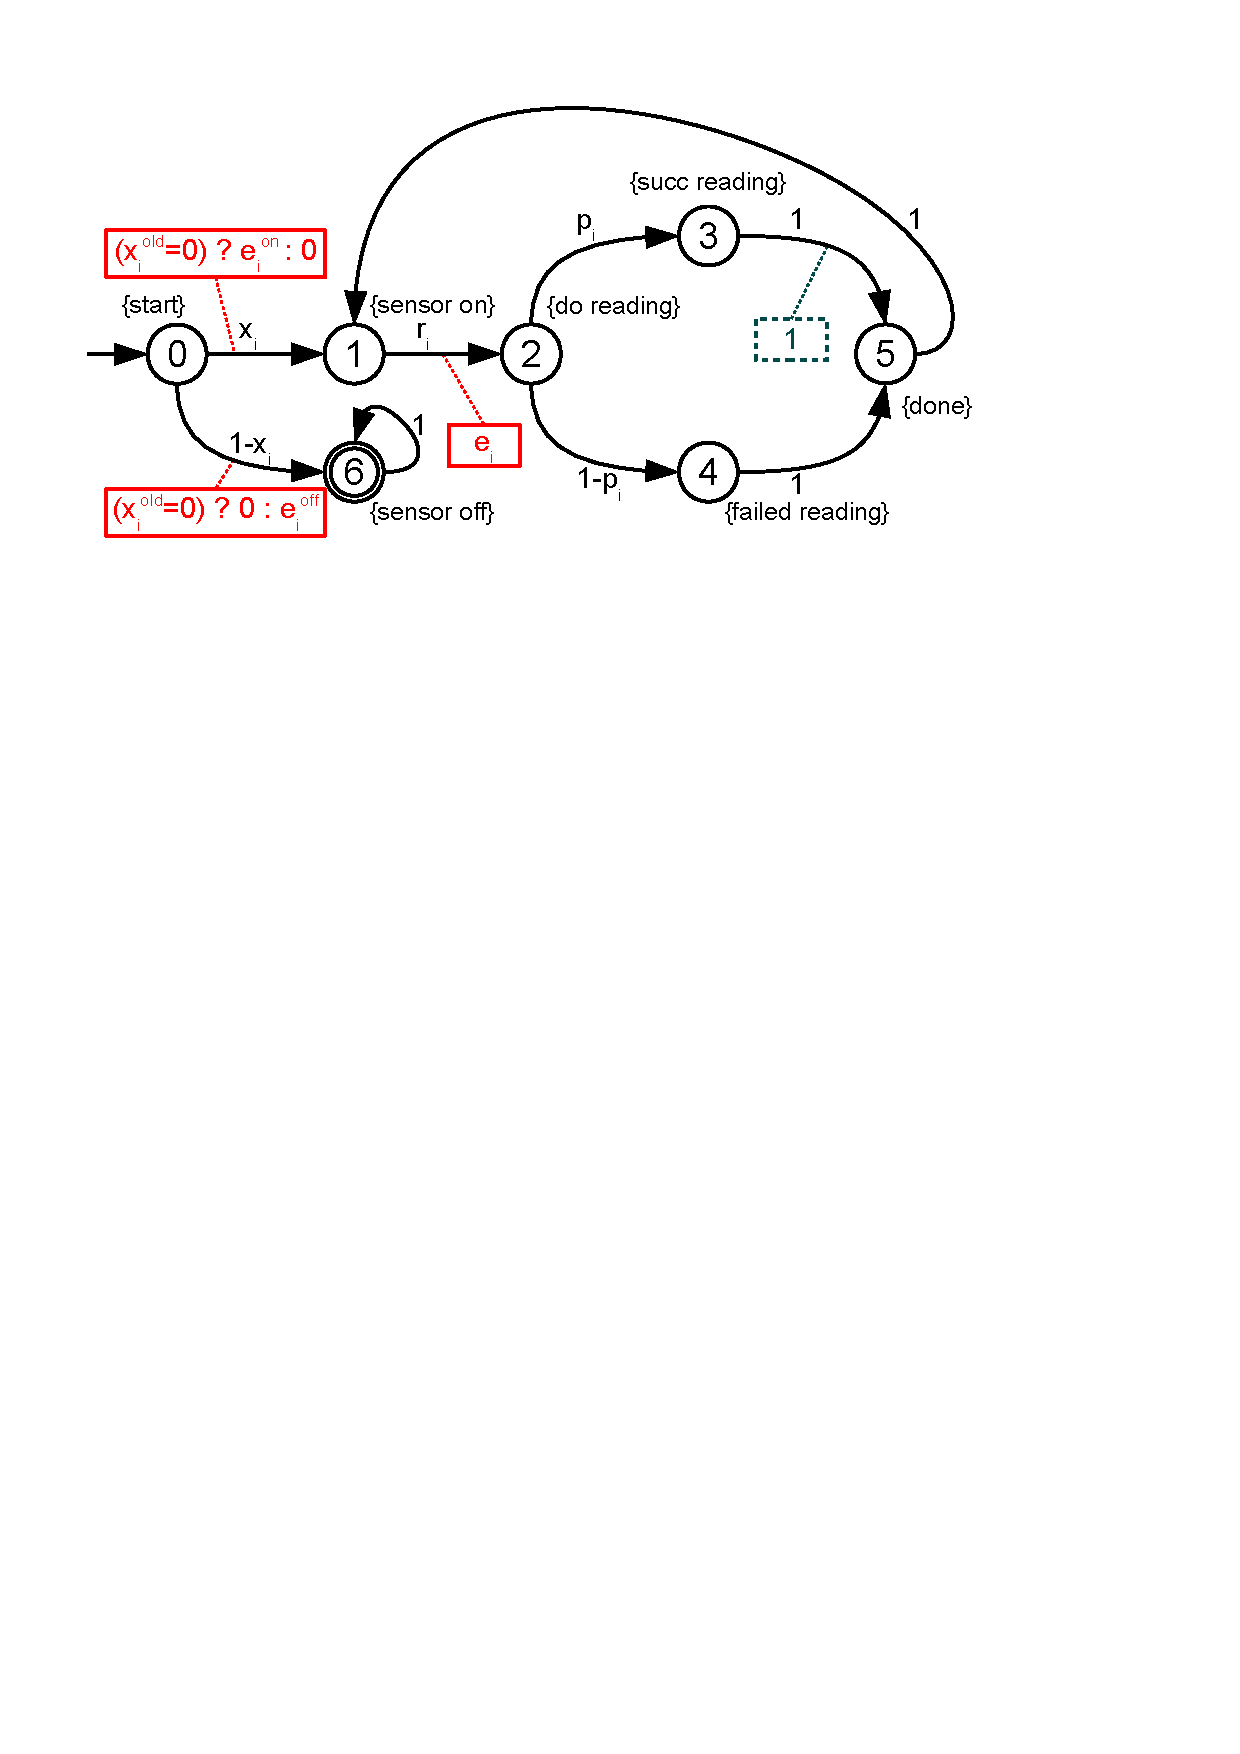
\includegraphics[trim = 17mm 205mm 45mm 17mm, clip, width=0.7\linewidth]{figures/model.pdf}
\caption{CTMC model $M_i$ of the $i$-th UUV sensor}

\vspace*{-2mm}
\end{figure}

\end{example}
